\chapter{SysML and Classical B}
\label{sec:sysML-B}

This section describes the approach of combining SysML modeling with
Classical B. The technical realization is shown in Figure~\ref{fig:classical-b-toolchain}.
Modeling starts in SysML based on the
tool Papyrus. At the current stage of the project, it is undefined
which SysML elements and diagrams will be used. This must be well
defined to ensure that a transformation from SysML to Classical B is
semantically correct. To validate the SysML model according to define
modeling guidelines, the approach suggest the use of the \emph{Object
  Constraint Language (OCL)} or the \emph{Eclipse Validation
  Framework}. Such guidelines may restrict the usage of certain
modeling elements and may enforce certain naming conventions.

\begin{figure}[b!]
  \centering
  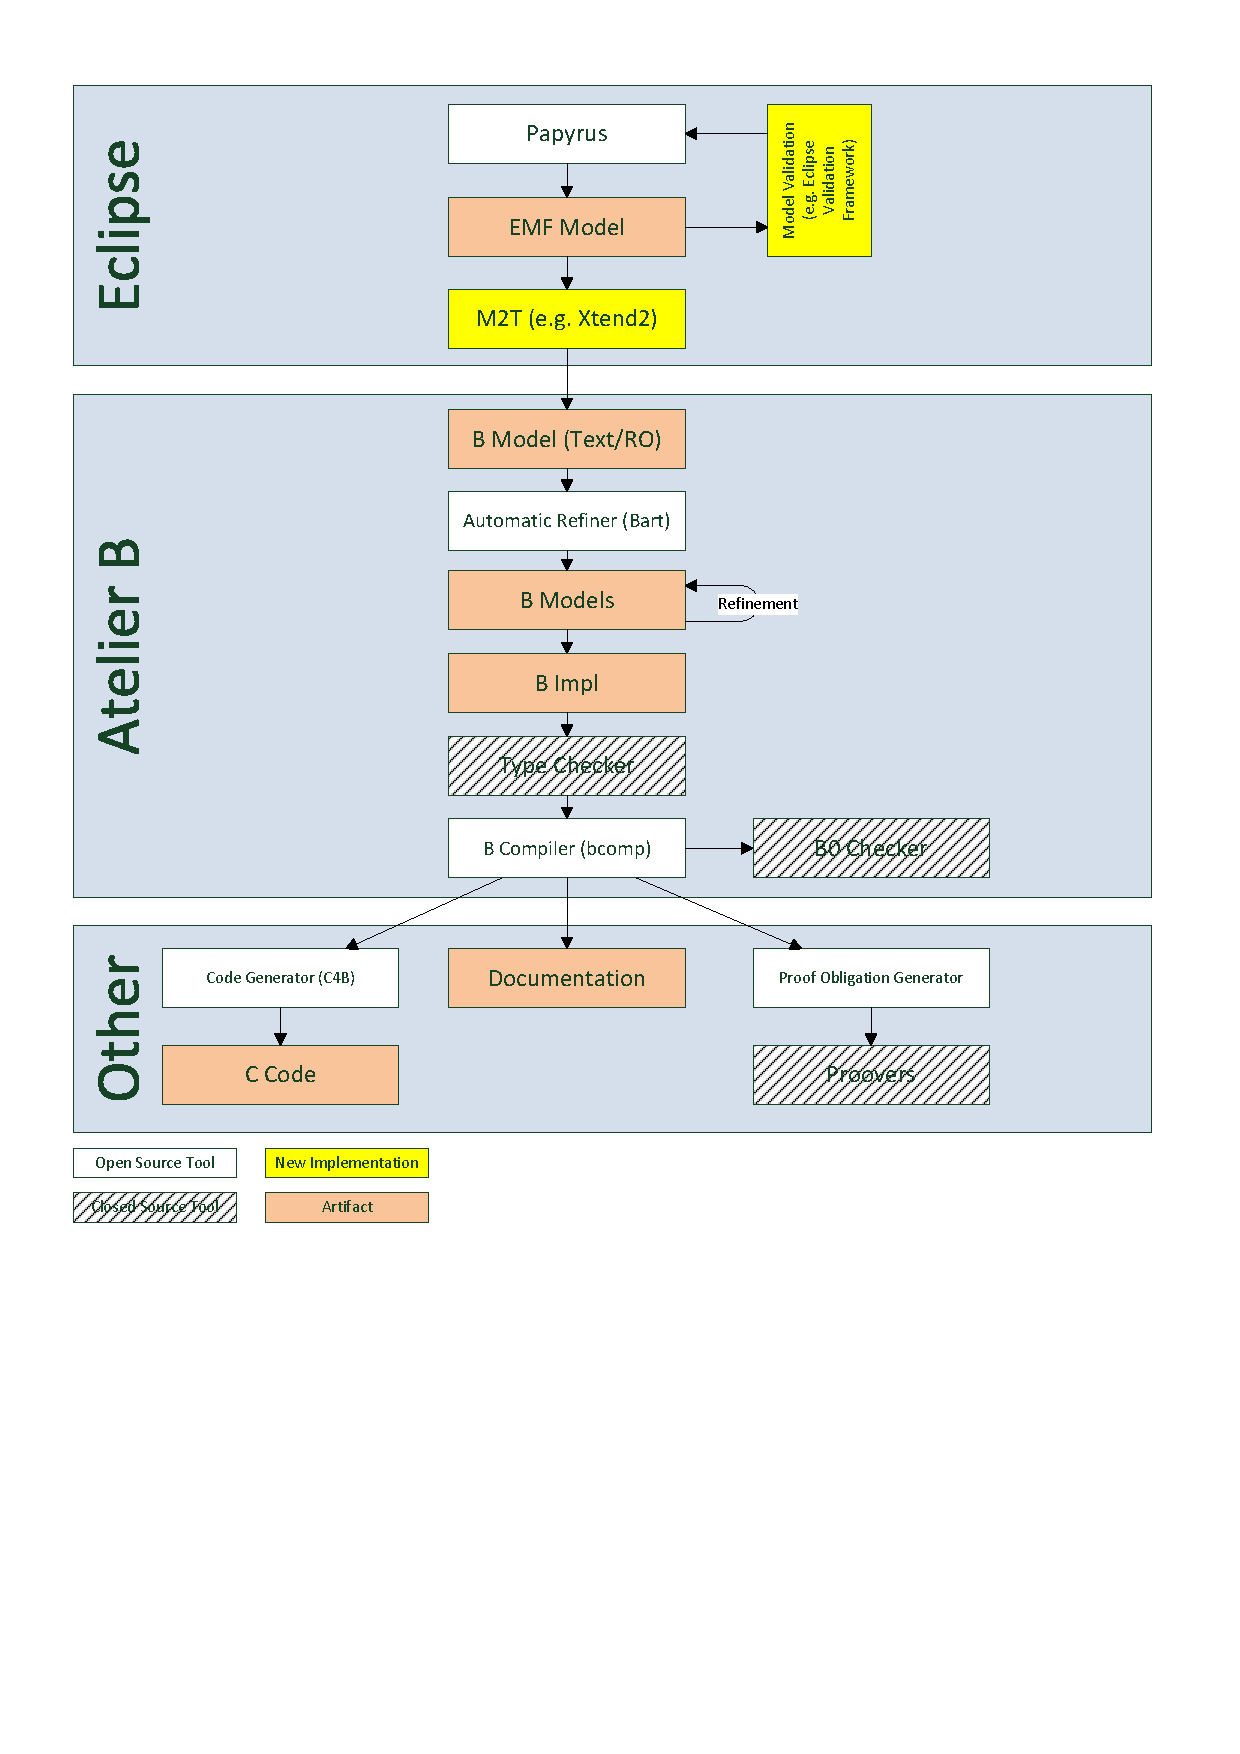
\includegraphics[width=6in]{images/classical_b_toolchain.pdf}
  \caption{Technical overview of the Papyrus and Classical-B toolchain}
  \label{fig:classical-b-toolchain}
\end{figure}

The validated SysML model will be transformed to a Classical B model
with a model-to-text transformation language (e.g. Xtend). The
generated Classical B model is considered as read-only and is only
allowed to be further refined. From that point, the existing Atelier B
toolchain will be used for refining the model until reaching the
implementation. Provers support the V\&V activities and the open
source code generator c4b is capable of generating C code. However,
the generated C code is not SIL4 certified. For SIL4 code generation,
there is the option to replace it with a commercial T3 translator or
to develop an own translator. As the software structure is closely
captured in the resulting B model, the translation from B to the
target language is less complex than it is the case with languages
that lack this strong relationship.

The proposed toolchain is intended to be a first version. The yellow
boxes in Figure \ref{fig:classical-b-toolchain} indicate non existing
software artifacts that have to be developed within the openETCS
project. Furthermore, it is desirable to move parts from the Atelier B
tool into Eclipse. 

In Table \ref{tab:classical-b-tools} the list of tools used in the
proposed toolchain is given. The GPLv3 licensed tools are stand-alone
executables. It is not expected that GPLv3 licensed tool will lead to
license issues with EUPL code, as these tools are only executed and
not linked with other parts of the toolchain. The ComenC code
generator is listed in the table, because the current version of
Atelier-B ships with it instead of c4b. The source code of ComenC is
available, however it is unclear under which license the source code
is distributed. The Type Checker, Checker, Prover and Proof Obligation
Generator are currently only distributed under a proprietary
license. However, with BEval and BWare (see Table
\ref{tab:classical-b-tools}) open-source alternatives are
available. BEval is a tool which allows verification of models by
model-checking with the ProB model-checker. In the BWare project a new
open-source proof obligation generator is under development. Both
tools could complete the toolchain to have open-source alternatives
for V\& V activities.

\begin{table}
  \begin{tabular}{ l | l | l }
    Tool                               & License & Link \\ 
    \hline \hline
    Bart (B Automatic Refinement Tool) & GPLv3 & \url{http://sf.net/projects/bartrefiner/} \\ \hline
    Atelier B GUI                      & GPLv3 & \url{http://sf.net/projects/atelierbgui/} \\ \hline
    Bcomp (B Compiler)                 & GPLv3 & \url{http://sf.net/projects/bcomp/} \\ \hline
    c4b (C Code Generator)             & GPLv3 & \url{http://sf.net/projects/c4b/} \\ \hline
    ComenC (C Code Generator)          & -     & \url{http://sf.net/projects/comenc/} \\ \hline
    BEval                              & EPL   & \url{http://github.com/ValerioMedeiros/BEval} \\ \hline
    BWare                              & -     & \url{http://bware.lri.fr/index.php/BWare_project} \\ \hline
    Papyrus                            & EPL   & \url{http://www.eclipse.org/papyrus/} \\ \hline
    Xtend                              & EPL   & \url{http://www.eclipse.org/xtend/} \\ \hline
    Type Checker                       & proprietary & - \\ \hline
    B0 Checker                         & proprietary & - \\ \hline
    Prover                             & proprietary & - \\ \hline
    Proof Obligation Generator         & proprietary & - \\ \hline
    \hline
  \end{tabular}
  \caption{Tools used in the Classical B toolchain}
  \label{tab:classical-b-tools}
\end{table}



\section{Description of the approach for OpenETCS design process}

Taking into account the results presented in Section
\ref{sec:results}, the proposed toolchain completely covers both, the
system phase as well as the software phase (see
Fig. \ref{fig:results}). SysML with Papyrus would be used for modeling
the SSRS on analysis level. The same tools will be used for the
sub-system semi formal model, which will be created during the
sub-system formal design phase. The SysML models will then be
transformed to Classical B models, with the intention to perform
further development steps according to the B method.

For both, the sub-system strictly formal model and the software
semi-formal model it is proposed to use Classical B. The development
of the B model will be done by further refining the read-only B
models, which was generated from the SysML model. It has to be
investigated where \emph{exactly} the transition between SysML and
Classical B will be done. In particular, it is currently unclear which
SysML language constructs and diagrams will be used that can be
transformed to Classical B. The structure described in SysML with
\emph{Block Definition Diagrams (BDD)} and \emph{Internal Block
  Diagram (IBD)} are obviously prime candidates for a transformation
to Classical B, but which behavior diagram will can be transformed is
still under investigation.

The last part of the development process is the code generation and it
is proposed to be performed with an existing code generator tool
(c4b).

\section{Integration of the approach with SysML/Papyrus}

On the technical side, the integration will be performed by utilizing
the EMF framework of Eclipse. With an appropriate transformation
language (e.g. Xtend), the SysML model can be transformed to a textual
representation in Classical B. Whether or not it is advantageous to
perform the transformation with an intermediate Classical B meta-model
and an a mode-to-model transformation (see
Fig. \ref{fig:classical-b-transformation-alternatives}) is under
investigation.

\begin{figure}[b!]
  \centering
  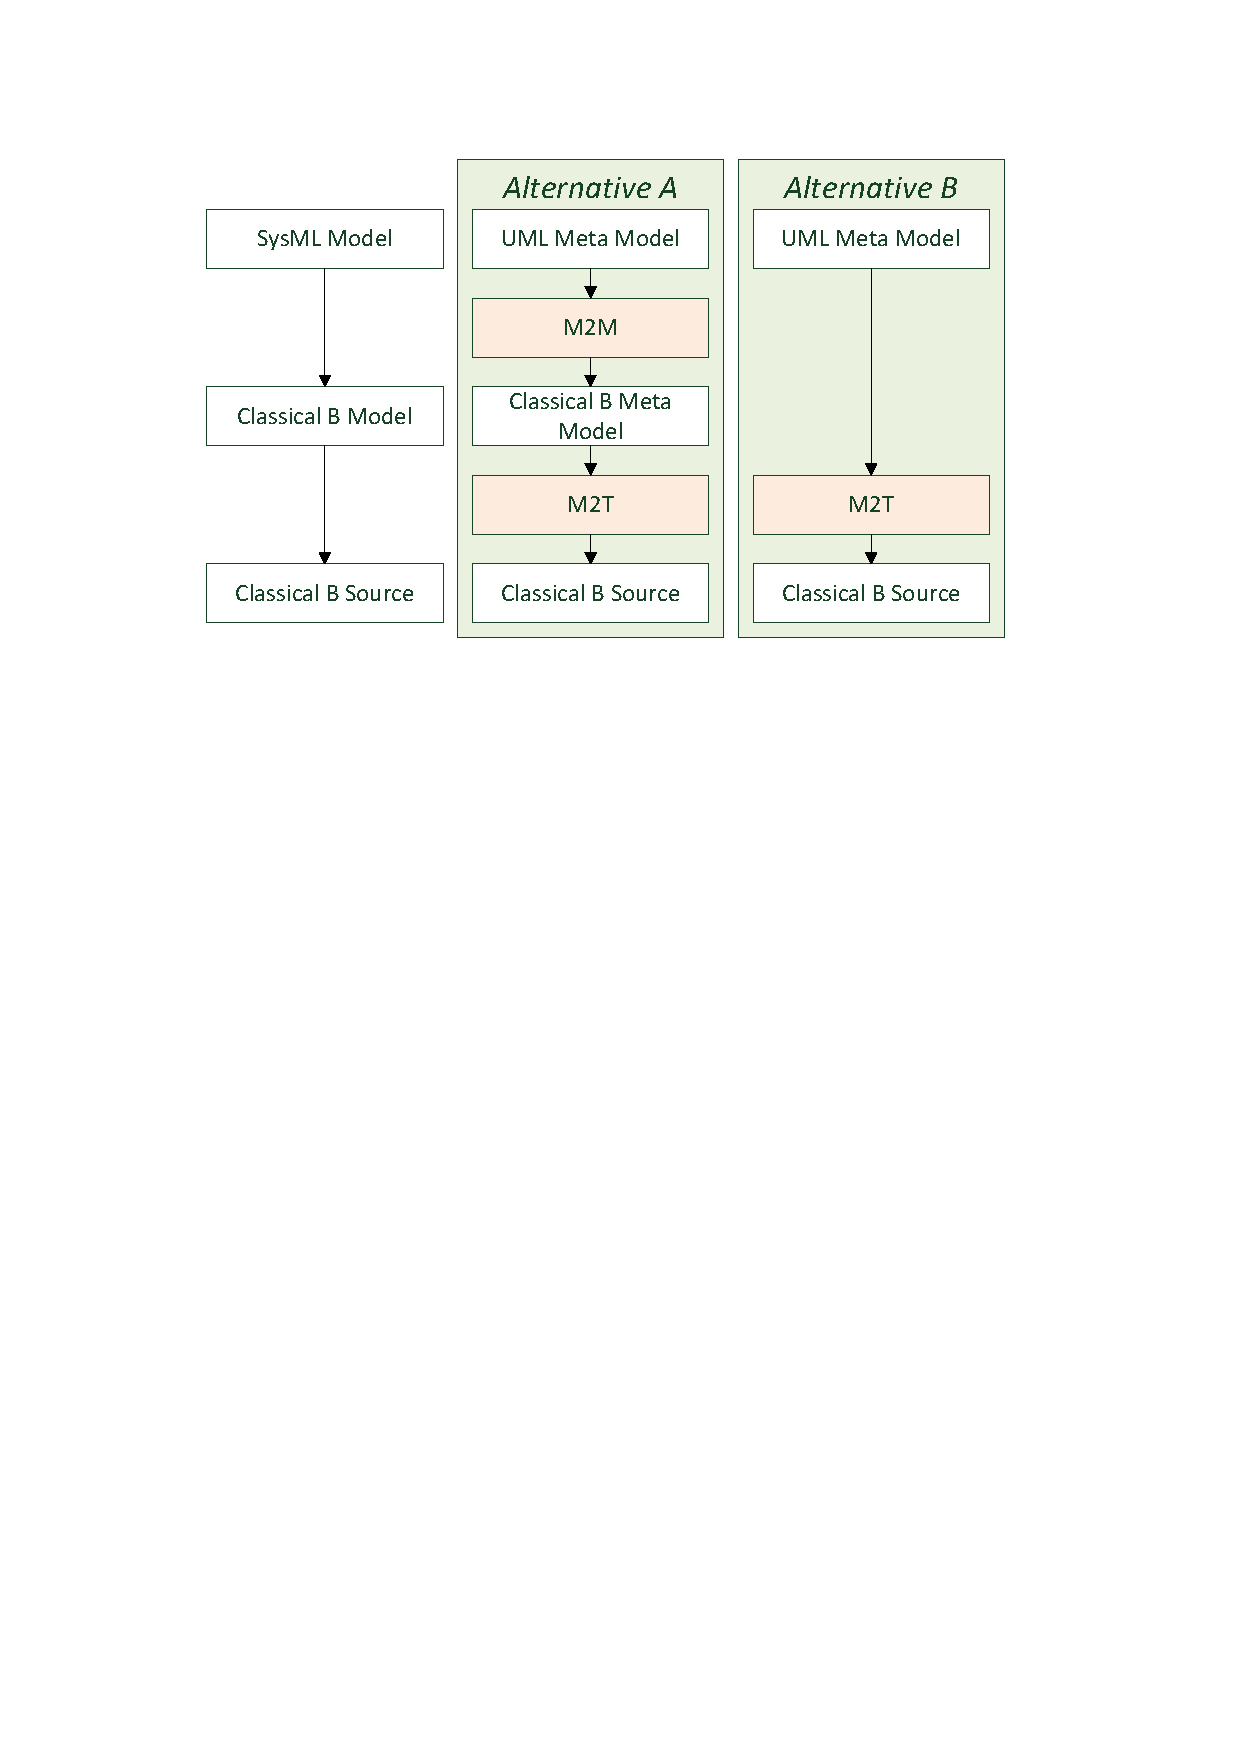
\includegraphics[width=4in]{images/classical_b_transformation_alternatives.pdf}
  \caption{Alternatives in the transformation from SysML to Classical B}
  \label{fig:classical-b-transformation-alternatives}
\end{figure}

The semantic integration of SysML and B method imposes a greater
challenge. There already exist literature regarding the alignment of
SysML and the B method. The work in \citep{bousse}
provides such an alignment focusing on V\&V, which could be used as a
base for further research, that considers in particular the openETCS
requirements.


\section{Integration of the approach with Eclipse}

The integration of the proposed toolchain is mainly done as described
in the previous section. After using SysML, the used tool is changed
to Atelier B. This obviously does not correspond to a fully Eclipse
based toolchain. However, this proposal only reflects an initial
toolchain, which could be improved during the project and beyond. The
parts of the toolchain which are user visible and realized with
Atelier B in the first version, could be progressively moved to an
Eclipse based solution. The open source tools involved in the
toolchain (automatic refiner, code generator, compiler, etc.) can be
executed from the command line, which allows an easy integration into
Eclipse. To what extend components from existing solutions (e.g. the
Rodin platform) can be used and if there are enough resources
available in the project, has to be investigated.

\section{Benefits versus OpenETCS requirements}

Both, SysML and the B Methods are accepted in the industry and have
been successful used in the development of safety critical embedded
systems. The B Method was used in projects like KVB by Alstom, SAET
METEOR or in the driverless metro line 1 in Paris by Siemens
Transportation Systems (see \citep{clearsy} for an extensive list).

Most parts of the toolchain are already available and distributed
under an open source license. The transformation from SysML to B is
the only missing software artifact, that has to be developed for the
first version of the toolchain (see
Fig. \ref{fig:classical-b-toolchain}).

The project consortium includes partner with great expertise in both
languages, SysML and B. By incorporating these expertise, there is a
good chance that the proclaimed goals of openETCS will be achieved.

The modular architecture allows the exchange of certain tools with
more powerful alternatives, even if they are closed-source. For
example, there is a closed source code generator which allows the
creation of ADA or C++ code. This code generator could be used as a
drop-in replacement for the open-source c4b if necessary.

Furthermore, with Eclipse and Atelier-B versions for Windows, Mac OS
and Linux, the most common operating systems are supported by the
proposed toolchain.

\section{Shortcomings versus OpenETCS requirements}

Although the majority of the toolchain is open-source, there is still
a small amount of tools which are closed source (see
Fig. \ref{fig:classical-b-toolchain}). During this project, these
parts will be further investigated with the goal to be replaced by
open-source equivalents.

A general weak point of the approach is the interface between Eclipse
and Atelier-B. It would be favorable if the tool flow is only
unidirectional. However, if during refinement steps in Classical B an
bug in the initial B model is encountered, a correction in the
original SysML model is necessary. This change triggers the generation
of a new, initial B model. A bi-directional transformation could ease
this issue, which would require a tighter integration of both
tools. This is amongst other one reason why moving parts from
Atelier-B to Eclipse should be further investigated. This issue
applies to all proposed toolchains as all change at a certain point
the modeling tool and the used language.

The example from the previous paragraph also show that the modeler
should preferable have knowledge of both, SysML and Classical B. The
reason is that otherwise bugs found in the SysML model during the
Classical B development phase have to be fixed by the modeler of the
original SysML model, which may be inefficient. This issue should be
also considered when the border between SysML and Classical B is
defined.

\section{On going work for openETCS project}

One of the most important parts is to define a subset of SysML which
can be transformed to Classical B and preserves it semantics. Probably
the other toolchains also need a restricted usage of SysML, therefore
a collaboration on this topic would be advantageous. Furthermore, it
would be ideal if one subset could be defined, which is applicable to
all proposed toolchains.

Another ongoing work is the precise definition of the border between
SysML and Classical B. This work is also linked to the work described
in the previous paragraph, as the border may have implication on
diagrams used in SysML.

The transformation from SysML to Classical B must be planned and
developed within this project. On the implementation part a desirable
skill is the knowledge of transformation languages in Eclipse.

Experience has shown that for model transformations the source model
should be checked according to guidelines. An obvious one is naming as
the source model may allow character combinations that are prohibited
in the destination model.

To show the capabilities and to identify any currently unforeseen
barriers, an early prototype should be developed which illustrates all
steps using an example use-case.

\section{Conclusion and other comments}

The proposed toolchain based on SysML and Classical B covers the
openETCS design phases from system analysis, sub-system formal design,
software design and software code generation. Furthermore, an
operational open source toolchain is already available from high level
B model design to C code.

Both, the proposed languages and tools have industry acceptance and
there exists a significant experiences in developing safety critical
system with such languages.

With the exact definition of the border between SysML and Classical B,
only the transformation between both languages has to be developed for
an initial version of the toolchain. During the project, this initial
version can be gradually improved to remove the last remaining
closed-source (see Fig. \ref{fig:classical-b-toolchain}) tools.
